\documentclass[../main-v1.tex]{subfiles}
\begin{document}
\chapter{Use Cases}
\label{ch:use}
\newcommand{\ignore}[1]{{}}



\section{Introduction \hideme{Schellman - draft}}

To introduce the \dword{tr} level processing issues for \dword{dune} computing, we describe some of the known use cases.  %We start 
This chapter starts with  the experience gained from  \dword{protodune},  using lessons learned from the 2018 run to understand the performance of future near and far detector modules. 

We note that, in addition to the challenges faced by \dword{hllhc} experiments, as described in the HSF White Paper\cite{HEPSoftwareFoundation:2017ggl}, DUNE (along with some dark matter and astrophysics experiments) faces considerable challenges in extracting very weak signals from large, noisy data volumes.  This additional challenge places strains on memory management beyond those anticipated at collider experiments. 

\section{Data Acquisition and Storage\hideme{Schellman - draft}}

\dword{daq} software and hardware are the responsibility of the \dword{daq} group, with significant interfaces to offline computing. Important factors include communication of calibration and configuration information between online and offline computing, high-speed networking for data, high-reliability networking for configuration and monitoring, and adequate disk and CPU on both ends of the connection to allow both efficient data transfer and continued data taking in the event of an extended network interruption. 

These considerations apply to \dword{proto}, where data taking occurs at the \dword{cern} with offline databases and archival storage in the US,  and, in the future, the far and near detectors in South Dakota and Illinois, respectively. 

Current status and proposed solutions are discussed in Chapters~\ref{ch:db}(Databases) and \ref{ch:netw}(Networking). 

\subsection{Data Transfer from the Experiment}
Data need to be buffered locally and then transferred to permanent storage at the host lab(s).  Transfer activities include the generation of descriptive metadata, file transfer, writing the files to permanent storage, and integrity checks.  Once data are confirmed to have successfully reached permanent storage, the local buffer may be cleared.  Current specifications call for the local buffers at remote sites to be able to store 3-7 days worth of data or one \dword{snb}'s worth ($\sim 500$ TB) at a minimum. 

%{\it Major concerns:  Network bandwidth and reliability between Sanford and Fermilab. The ability of host lab systems to absorb and redistribute those data quickly. }
{\it Major challenges: Here the major areas of concern are the remote location of the far detector, and space and power limitations at both the \dword{4850l} detector level and the surface. %anne Other challenges include 
Another challenge is the need for adequate lossless data compression to prevent data volume explosion. Chapter \ref{ch:netw} describes the status and plans for networking.}

\subsection{Control, Configuration, Conditions and Calibrations}
%\subsubsection{Configuration and Monitoring}
In addition to large-scale data transfers, online data-taking configurations and conditions need to be stored and communicated to the offline systems. High-reliability network connections are needed to ensure that control signals, and configuration and monitoring information are exchanged between the remote sites, local control facilities and the host laboratory.
This is the responsibility of the \dword{fnal} networking groups and the \dword{daq} consortium with input and assistance from offline computing. 


\subsubsection{Slow controls}
Data from slow control and monitoring systems need to be recorded for offline use.  Examples include set points and readback for \dword{hv}, %anne systems, 
pressure, temperature and the outputs of purity monitors. 

{\it Potential challenge: Commercial \dword{scada} systems tie us to proprietary software that may have limited interfaces, require expensive licenses and need migration to new systems if %the vendor stops support.
vendor support becomes unavailable.}

\subsubsection{Online Calibrations}
Online calibration information (e.g., pedestal information) needs to be passed to the offline systems. 

%{\it No novel concerns.}

\subsubsection{Beam Monitors}
Beam monitoring information, either per spill for neutrino interactions or per particle in the \dword{cern} test beams, needs to be recorded and made available for offline processing. 
The \dword{ifbeam} system used for \dword{numi} is already in use for \dword{protodune}.

\subsection{Monitoring Information} 
Local online monitoring of data and experimental conditions will be done by the \dword{daq} %anne groups 
consortium, but fast feedback on data movement and quality will also need to be provided based on fast processing of a subset of the data transferred offsite. \todo{anne: Computing will provide this?}

{\it There are no novel concerns, but substantial effort will be needed to build and maintain the system over the lifetime of the experiment.}

\subsection{Offsite High-level Data Filtering}

This is not yet part of the data plan but there may be a need for offsite filtering of data before %anne it is 
it is written to permanent storage. 

{\it  Initiation of a high-level trigger offsite remains a possibility if the need arises. Local space, power and cooling issues make this difficult to do at \dword{surf}.}

\subsection{Data Compression}
In \dword{pdsp} lossless compression was performed as part of the \dword{daq}. For \dword{pdsp2} this is not planned due to the need to keep processing overheads low in the \dword{daq}. Lossless compression will need to be applied later in the processing chain, most likely using the intrinsic compression methods of the chosen data format(s).  \dword{root} allows implementation of lossless compression, as does \dword{hdf5}.


\subsection{Outputs from DAQ and monitoring}

At the end of data transfer and after acquisition of configuration information,  %anne we assume 
it is assumed that data, metadata and configuration/calibration/beam information from the detectors will have been transferred to offline computing facilities and can then be distributed and reconstructed. 

\section{Supernova \hideme{Schellman/Kirby - needed}}


\section{Simulation Chain \hideme{Junk and Schellman - draft}}

% 
The simulation chain involves multiple steps.

\subsection{MARS}
The \dword{mars}\cite{abs1} simulation is used in the design of the beamline and near detector systems and  for safety and environmental calculations.  It is a significant user of CPU time. 

{\it Unique challenge: the \dword{mars}\ codes are not available outside of \dword{fnal}.}

\subsection{Beam Simulations}
The \dword{lbnf} 
beamline is simulated using the \dword{g4lbnf} framework.  The \dword{proto} beamlines were designed and simulated using the MAD-X framework used at \dword{cern}\cite{PhysRevAccelBeams.20.111001}.
Inputs include random number seeds and the beamline and target region geometry and materials.  Outputs are flux files containing simulated neutrino trajectories.  The flux files contain sufficient information to allow reweighting based on interaction cross sections.  These flux files must be catalogued and made available to offline simulation jobs.

{\it Minor challenge:  Distribution of flux files to remote sites requires use of \dword{stashcache} and careful record keeping.}



\subsection{Neutrino Event Generation}

Extracting physics results from the DUNE experiment requires comparing the observed data with simulations %anne, which include detailed simulations 
of the physics processes under study as well as of the response of the detectors.  The physics simulation is performed by the neutrino generators \dword{genie}~\cite{Andreopoulos:2009rq}, NuWRO~\cite{NuWro2012}, GIBUU~\cite{Gallmeister:2016dnq}, NEUT~\cite{Hayato:2009zz}, and others. 

Neutrino event generators are used to simulate neutrino interactions within a detector volume.  Input requirements are the neutrino beam flux, random number seeds and the detailed detector geometry. The output consists of four-vectors for final-state particles, including short-lifetime decay chains.  DUNE currently uses \dword{genie}~\cite{GENIE} as the default, but other default generators are possible. 

\subsection{Non-Beam Interaction Simulations}
Simulations of non-standard model physics (e.g., neutron decay) and of cosmic ray and rock muon backgrounds are also used.  Cosmic ray simulations are performed with \dword{corsika}~\cite{Wentz:2003bp,Dembinski:2020wrp} for detectors on the surface, and MUSUN/MUSIC for detectors deep underground~\cite{Kudryavtsev:2008qh,LBNEDOCDB9673}.  Radiological decays are modeled with BXDECAY0~\cite{Ponkratenko:2000um} and the DUNE-specific RadioGen.

Factorization of the simulation into a generation stage and a detector simulation stage is a common situation \todo{anne: a common step?} in collider experiments, such as ATLAS and CMS.  The fact that the interactions simulated by generators for collider physics happen inside an evacuated beampipe means that the details of the detector geometry and materials are not relevant for most event generation, and lists of four-vectors of particles emerging from a primary vertex will suffice.  In a neutrino experiment, however, the detector material is the target material, and hence the generators must be aware of the detector geometry and materials, which affects the structure and performance of the generator code.  Currently \dword{genie}, \dword{corsika}, MUSUN/MUSIC, BXDECAY0 and RadioGen are integrated with \dword{larsoft}.  \dword{genie} is also integrated with \dword{garsoft}.

{\it We can rely on strong international efforts to produce standard generators. One challenge is the complexity of integrating multiple simulation code versions into our framework to ensure that there is timely evolution of the generators used as the physics understanding evolves.}

\subsection{Detector Interaction Simulation}

Two classes of detector simulation for DUNE exist at the time of writing. 

Parameterized, or ``fast'' detector simulations involve smearing truth-level physics quantities based on expected detector performance metrics, such as acceptance and energy resolution.  These fast simulations are useful when optimizing detector designs, and for engaging physicists outside of the DUNE collaboration.  

\subsubsection{Full Detector Simulation} 
Full simulations, on the other hand, are based on detailed geometry models and \dword{geant4}~\cite{Agostinelli:2002hh,Allison:2016lfl}, and are needed for extraction of publication-level results.

A detector simulation such as GEANT4~\cite{Allison:2016lfl} or FLUKA~\cite{Bohlen:2014buj} is used to simulate the interaction of the particles described by the four-vectors produced by the event generator. Input requirements are the geometry and outputs are the tree of interactions and energy deposits in the active detector materials. 
Energy thresholds need to be quite low, as the detector systems are sensitive to MeV-scale processes. The large uniform detector volumes in \dword{lar} detectors compensate for the low thresholds by requiring fewer volume crossings in a typical particle trajectory.  

Hadronic cross section on \dword{lar} are not yet fully understood.  DUNE has developed a reweighting framework 
\dword{Geant4Reweight}~\cite{Calcutt:2021zck} to allow reuse of existing simulation as interaction rates are refined.

{\it Major concern: Due to the high granularity and low energy thresholds, interaction records can become very large. Simulated \dword{protodune} records are currently 200-300\,MB, substantially larger than the raw waveforms.}

\subsection{Detector Simulation}
\Dwords{lartpc} require detailed models of electron trajectories through a potentially charged fluid.  Photon detection requires ray tracing over long distances.  Once electrons and photons have been propagated to the detection systems, simulation of the electrical response must also be done. Inputs are the output of the detector simulation, charge distribution in the liquid, absorption parameters and the detailed readout system geometry. Outputs are simulated streams of bits in the electronics. 

The propagation of low-energy drifting electrons and scintillation photons, signal induction  and electronics response are then simulated in a separate step.  

A large amount of code re-use and sharing via the design of \dword{larsoft} allows for the development of simulation algorithms for \dword{pddp}, the dual-phase far detector, 
\todo{anne: keep reference to DP?}
and the \dword{spvd} detector proposals.  Only the geometry, the field description, and the anode plane models need to be updated; the rest of the simulation chain is re-used.

\subsection{TPC Simulation}

Drifting electrons are simulated parametrically using a model based on the measured drift velocity, longitudinal and transverse diffusion coefficients, and a parameterized model of space charge.  This last effect is particularly pronounced at \dword{pdsp} due to the large number of cosmic rays crossing the detector volume, giving rise to distortions in the apparent positions of particles of up to 30\,cm.  % anne There are also field distortions due to e
External imperfections such as the grounded electron diverters in \dword{pdsp} also cause field distortions.

Once the electrons drift to the anode plane in wire-based \dwords{lartpc} in the simulation, a detailed \twod model of the wire responses is applied~\cite{Abi:2020mwi}.  The two dimensions are wire number and time, and the effects of induced currents on neighboring wires are included in the simulation.  The electronics response function is folded in to a final model of the observed waveforms.  Simulated waveforms have been compared with real ones  in \dword{pdsp} and are found to be very similar.
In the pixel-based \dword{ndlar} and \dword{ndgar}, the electronics simulation is at a simpler level, as the electronics have not been fully designed.

\subsection{Photon Detector Simulation \hideme{Paulucci - draft}}

Photon simulation in large detectors is known to be highly computationally intensive due to the need to trace large number of photons over large distances.  \dword{dune} has several approaches to this problem. 

The sequence for photon simulation is:
\begin{enumerate}
\item perform particle track simulation in \dword{geant4} to produce the energy deposits along the track;
\item  calculate the number of photon/electron emission at each vertex where energy deposits; \item 
simulate the photon transport in the detector (either full simulation or fast simulation); and
\item  reconstruct the photons, including the hits and flashes. %anne reconstruction
\end{enumerate}
 
In \dword{larsoft}, after particles are propagated using \dword{geant4}, energy deposits along tracks are recorded so that the number of electrons and photons generated at each step can be estimated using one of the available  ionization and scintillation methods. Once the number of photons is determined, the fraction of those photons that will actually reach a given photon detector is usually estimated using one of several fast light-simulation methods. This procedure is followed for both 128\,nm photons (Ar scintillation) and 176\,nm photons (Xe scintillation) to account for the wavelength-dependent Rayleigh scattering in the simulation of Xe-doped \dword{lar}. 
Since a copious number of scintillation photons (25000\,ph/MeV at 500\,V/cm) is produced in \dword{lar}, it is very demanding computationally to propagate all photons individually using \dword{geant4}. Instead,  fast simulations for photons are implemented.
%The photon simulation CPU time per event which depends on what kind of events are simulated and the simulation methods. 
The full \dword{geant4}  photon simulation CPU time per event depends on the energy deposited. 
In the fast simulation methods, using a library,  semi-analytic methods or machine-learning, the CPU time depends on the granularity of the detector. Generally speaking, the performance of the three fast simulations methods is similar. %anne at the same level. 
 
\subsubsection{Optical Library Method}

This method consists of dividing the cryostat volume into smaller parallelepiped-shaped regions called voxels and creating a lookup matrix %anne table 
(the optical library) %anne that can store the visibility of each photon detector to photons being generated inside a given voxel.
in which the cells store the capability of each photon detector to detect photons generated inside each voxel.
This optical library is created using the full \dword{geant4} simulation to generate photons anywhere inside a given voxel, with random direction and polarization, and then store the fraction of those photons that land on the optically sensitive region (visibility) of a given photon detector, identified within \dword{larsoft}  by its optical channel. When using the fast simulation, \dword{larsoft}  will retrieve the Optical Library and store its information to directly transform the number %amount 
of photons generated in a given step along a particle's track into the number of photons landing on each optical channel.
This method can %anne satisfactorily 
be used as a fast simulation method, but %anne. Nevertheless, 
its performance greatly depends on the size of the voxel and the number of photons being generated per voxel. Increasing the number of voxels in a library will improve the description and reduce the bias at the cost of a large increase in memory consumption. Increasing the number of photons per voxel will provide much better statistics and also largely increase the amount of time dedicated to generating the optical library. Special care should be taken for regions with %anne smaller
lower visibilities.

\subsubsection{Generative Neural Networks}

%Fast simulation with Generative Neural Network
This method relies on a generative neural network  trained on the detector's \dword{pds}. %anne photon detection system of a detector. 
The input to the network is the vertex where the photons are emitted, and the output is the visibility of each photon detector. \todo{anne: 'visibility' is the ability to be seen, not to see; replace with something like 'detection capability'?}
The generative model can be trained ahead of time using a full  \dword{geant4} optical photon simulation with photons emitted from random vertices in the detector, after which it can be frozen to a computable graph and deployed to the production environment (\dword{larsoft}  framework).

When the computable graph is loaded in \dword{larsoft}, it quickly emulates photon transport by  computing the %anne visibility 
detection capability of each photon detector according to the photon emission vertex along the particle's track.
This method is 20 to 50 times faster than the \dword{geant4} simulation while keeping the same level of detail for particle tracks, such as the number of energy depositions and the precision.
The model inference also requires a relatively small amount of memory. The samples for \dword{protodune}-like and %anne DUNE-like 
far detector-like geometries show the required memory for the model inference is around 15\% of the \dword{geant4} simulation. Further, this memory use is not directly correlated to the volume of the detectors. \todo{anne: is the GEANT4 directly correlated to vol?}

\subsubsection{Semi-analytical Models}
A large number of photons is generated at different points within the cryostat volume and propagated using \dword{geant4}. Gaisser-Hillas functions are fitted to the %anne number of 
photons reaching the photon detectors as a function of source-detector distance and relative angle, and the resulting parameters are used during event simulation %anne in order 
to extract the fraction of photons produced at a certain point that arrives at a given sensor.
 
\subsubsection{Comparison between Fast Simulation Methods}
The semi-analytic model and the use of  optical library models for fast simulation have been compared to the full light simulation in \dword{geant4} for the \dword{sbnd} experiment. This used a highly segmented and large-photon-count optical library, created with $\sim$1.6M voxels, with 0.5M photons %anne being 
generated in each voxel (total of $7.9 \times  10^{11}$ photons), resulting in a  1.2\,GB file size. A similar optical library for the DUNE 1$times$2$times$6 geometry (volume of $7 \times 12 times 13.9$ m$^3$) would be prohibitively large.
All DUNE optical libraries produced so far have larger voxels and fewer photons simulated per voxel %anne being simulated in comparison with the
than \dword{sbnd}, one library of which \todo{anne: check, I think 'library' is right} was used as reference for the comparison of the two modes. It has been reported that the optical library struggles to properly describe light signals generated closer to the detectors and more on-axis (up to $\sim50\deg$). This is a known issue caused by the intrinsic discontinuity of the voxelization schemes. In the \dword{protodune} optical library, %a smoothing of visibilities using neighboring voxels was used trying to minimize this effect. 
we tried smoothing the detection capabilities over sets of neighboring voxels to minimize this effect.
\todo{anne: did it work?}

The semi-analytic model, on the other hand, presents a reduced resolution when going off-axis due to shadowing effects. The influence of shadowing should be minimal for the case of %anne DUNE FD 
the \dword{fd} as there are no \dwords{pmt} in the geometry (in \dword{sbnd} the \dwords{pmt}' windows %anne reach out to 
extend about $\sim$10\,cm beyond the \dword{xarapu} windows), so %anne in the DUNE case we 
DUNE expects  good performance of this %the semi-analytic 
model even in the far-off-axis cases.
%anne Specifically for the \dwords{xarapu} in \dword{sbnd},  b
Better performance of the semi-analytic model is expected for the \dwords{xarapu} in \dword{sbnd}: better resolution close-on axis (3.6\% vs 5.6\%), with no bias (less than 1\%) in any case \todo{anne: meaning on or off axis?}, while the optical library is systematically biased (2.5-4.9\%), in particular for the larger/closer signals. This, together with the very high memory consumption (several extra GB) during simulations when using an optical library, justifies the current choice of the semi-analytic model as the default for fast simulations in the DUNE \dword{fd}.




{\it Challenges:  \dword{protodune} experience indicates that, although simulation is reasonably fast relative to reconstruction (3 to 1), memory utilization %anne even for \dword{protodune} 
is very high in simulation jobs.  Process sizes of 5-6\,GB in memory are typical for six \dwords{apa}.  High energy \dword{fd} interactions are expected to span more detector volume and thus require even more memory. Multiple \todo{anne: simulation?} passes may be needed since optimization of the electron trajectory model is recursive and generally requires multiple reconstruction passes. }

\subsection{Near Detector Simulations\hideme{Junk and Muether - needs more}}
The \dword{ndgar} detector also has a calorimeter and a muon system.  The calorimeter is currently simulated via parameterized responses to the \dword{geant4}-simulated energy deposits, as are the responses to tracks in \dword{ndgarlite} and \dword{sand}.

\subsection{ProtoDUNE Simulation Experience\hideme{Yang - draft}}

The detector simulation framework has already been tested successfully in \dword{protodune}. 

The \dword{pdsp} simulation includes beam particles, cosmic ray interactions and radiological backgrounds. The beam particle species and momentum distributions are from the \dword{geant4} simulation of the H4-VLE beam line at CERN, which consists of $e^{+}$, $\pi^{+}$, $p$, and $K^{+}$ particles at 0.3, 0.5, 1, 2, 3, 6, and 7\,GeV/$c$. Cosmic ray interactions are produced with the Corsika generator. Radiological backgrounds, including $^{39}$Ar, $^{42}$Ar, $^{222}$Rn, and $^{85}$Kr, are also simulated using the RadioGen module in \dword{larsoft}. The primary particles are tracked in the \dword{lar} using the \dword{geant4} package. 
The ionization electrons are drifted towards the wire planes %anne. The 
and the effects of recombination, attenuation and diffusion are simulated. The accumulation of positive ions in the detector modifies the trajectory of ionization electrons and the strength of the \efield, which is known as space charge effects, and is simulated using the measured distortion and \efield maps. The electronic signal is simulated by convolving the number of electrons reaching each wire plane with the field response and electronics response. The field response is modeled using the \dword{garfield} package. 
\todo{anne: I added the dword; add the definition please } The electronics response uses the parameterization from the \dword{spice} simulation with the average gain and shaping time measured in the \dword{protodune} charge injection system. 
\hideme{cite the papers for protoDUNE}
%Each event corresponds to a 3 ms readout window with a sampling rate of 0.5$\mu$s per time tick.  The total number of electronic channels is 15,360. 




\subsection{Overlays}
An efficient method for accurately simulating backgrounds in high rate environments is to overlay the simulated interaction information on real data.  For example, the environment in \dword{protodune} or the near detector includes multiple beam and rock muon interactions in the same readout as %anne (made plural) an 
the interactions of interest.  Libraries of properly formatted raw data can be combined with simulated hits from a simulated event to yield a realistic simulation of an interaction in the real detector. This requires a library of such interactions and careful matching of the running conditions of the external raw events to the desired simulated events. 

{\it Challenges: We have not yet integrated overlays into the experiment framework. To do this we will need to distribute large volumes of overlay data to remote sites while maintaining randomness. Other experiments such as MicroBooNE and MINERvA have done this successfully. }

\subsection{Reweighting}
If intermediate simulation steps  are stored they can be used to reweight interactions to reflect new knowledge about the underlying cross sections, neutrino flux, detector materials or detector properties. Examples include the \dword{ppfx} beamline simulation reweighting system and the implementation of different cross section and final-state interaction models in event generators. 

{\it This is not a major challenge, several reweighting packages have been developed for NuMI/DUNE \cite{Aliaga:2015wva, Calcutt:2021zck}.}

\subsection{Outputs from Simulation}
At this point we should have simulated data that is equivalent to the raw data coming from the detector. The next step is calibration and reconstruction. In all cases descriptive metadata needs to be produced that would allow reproduction of the simulation. 

{\it Possible challenge:  How many and which intermediate steps need to be stored permanently in order to optimize storage vs CPU utilization?}



\section{Reconstruction\hideme{Junk, Muether and Schellman-draft}}

%%%%%%%%%%%%%%%%%%%%%%%%%%%%%%%%


%\section{ProtoDUNEdata: raw data acquisition, cataloging and storage \hideme{Schellman - draft}}\label{sec:use:pdii-daq}



% \subsection{DAQ to Raw Data store \hideme{Schellman-draft}}
% The \dword{daq} and \dword{cisc} systems are expected to provide in close to real time:

% \begin{itemize}
%     \item Raw data from the \dword{tpc} and \dword{pd} detectors. 
%     \item Information on run and trigger configuration
%     \item Beam information
%     \item Information on detector conditions. For example, granular information on the \dword{hv} is needed to study and compensate for \dword{hv} fluctuations. 
%     \item Low level calibration constants such as gains that do not need extensive offline processing
    
% \end{itemize}


% The raw data are written to disk locally and then copied to the archive site (FNAL). Once the data are confirmed to be on tape, the local copy may be deleted.

% A second copy of the raw data will be stored in a different archive. 

% \subsection{Inputs to reconstruction}

% The run and trigger information, beamline  data, conditions and calibration constants are made available through separate data paths and stored in appropriate databases. In ProtoDUNE Run I, some of this information was transferred manually and stored in the \dword{sam} catalog.  DUNE document 22983 \cite{bib:docdb22983} describes the metadata strategy for ProtoDUNE II and DUNE. 

%Figure \ref{fig:ch:use:pdii} illustrates a typical reconstruction flow for ProtoDUNE data
\begin{dunefigure}
[Data flow diagram for standard ProtoDUNE reconstruction]
{fig:ch:use:pdii}
{Data flow diagram for standard ProtoDUNE data reconstruction. The central boxes show the processing steps while the right side shows the large scale data flow  and the left side shows the auxiliary information needed for processing. Thicker lines indicate particularly large data volumes.}
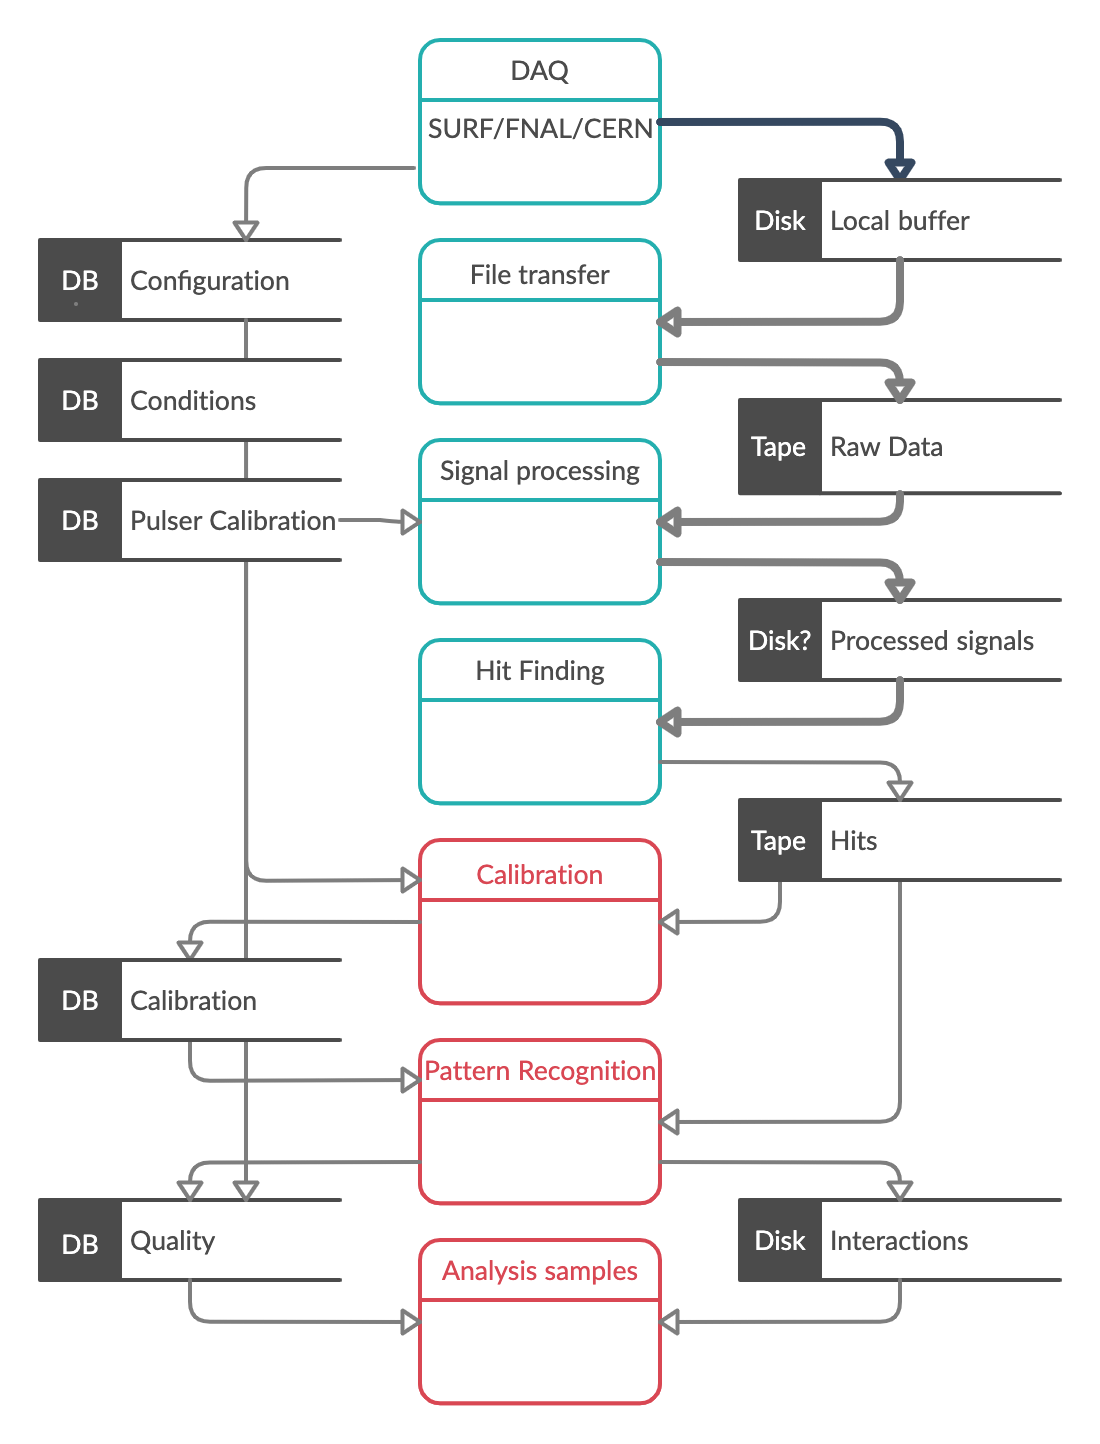
\includegraphics[width=0.8\textwidth]{graphics/IntroFigures/Data_processing_FD_v3.png}
\end{dunefigure}

\subsection{ProtoDUNE and Far Detector reconstruction\hideme{Schellman-draft}}\label{sec:use:pdii}

Figure~\ref{fig:ch:use:pdii} shows the data flow for regular reconstruction in \dword{proto}.  %anne There are in principle multiple stages in reconstruction that 
In principle, multiple stages in reconstruction are well suited to different computer architectures.  We expect the full \dword{fd} data processing to follow a similar path to that used by \dword{protodune}.  

Figure \ref{fig:ch:use:fdagg} illustrates  readout structures for full DUNE \dword{fd} modules.  A readout consists of a large number (up to 150) of   30\,MB \dword{apa} readouts and a number of smaller readout fragments.  These need to be processed and  recombined into a single readout record. 

\begin{dunefigure}
[Data aggregation diagram for FD]
{fig:ch:use:fdagg}
{Data aggregation cases for the far detector. The top case shows information for normal beam or calibration readouts. A single file of $\sim 10$\,GB size contains several complete \dword{tr} with their boundaries designated by the dashed lines.  \dword{tpc} \dword{apa}'s, \dwords{pd},  trigger primitives and a trigger  are recorded for each trigger readout.  In addition, a manifest, which describes the relations between the data, is stored either in the file or in external metadata.  The bottom case is a \dword{snb} readout, in which thousands of 5-10\,ms time slices must be read out over 100\,s.  The solid lines denote file boundaries. How data are ordered, by geographical position or by time,    is not  yet specified.}
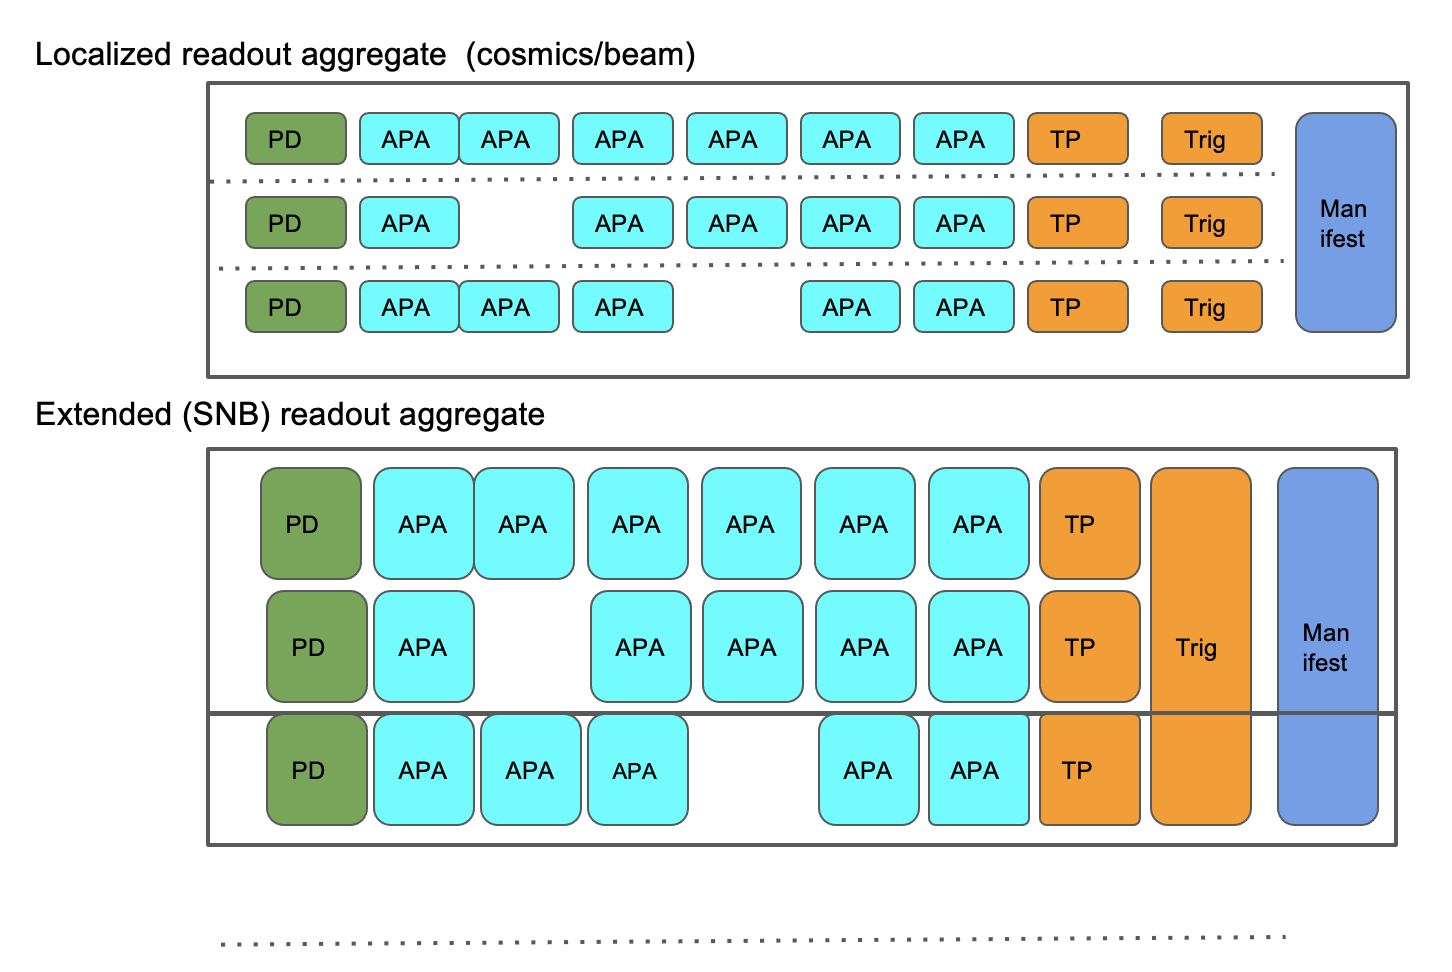
\includegraphics[width=0.8\textwidth]{graphics/IntroFigures/DataAggregation.png}
\end{dunefigure}
%\pagebreak

\subsubsection{Signal processing \hideme{Schellman-draft}}

Reconstructing events in a \dword{lartpc} is challenging.  Each trigger record contains a large number of waveforms, one for each readout channel.  In \dword{pdsp}, the waveforms typically were 6000 time ticks long, with one \dword{adc} sample per time tick.  A detailed description of the reconstruction procedures, starting with these waveforms, is given in~\cite{Abi:2020mwi}, and summarized briefly here.


The signal processing step takes the raw waveforms, applies  basic channel-to-channel calibrations, removes noise and stuck bits, and performs 1D or \twod deconvolution.   In the \dword{tpc}, this processing step operates on large \twod data arrays and may be suitable for different architectures than conventional pattern recognition. For the \dword{pd}, 1D data arrays will be the input. It is anticipated that the signal processing step will not need to be done frequently. 

The input data at this point are quite uniform, effectively bit streams from \dword{tpc} and \dword{pd} channels.  There are correlations between channels in the \dword{tpc} data that require concurrent processing of multiple channels.  Segmentation at the level of a readout plane within an \dword{apa}  or \dword{lem} is desirable.  An uncompressed input \dword{apa} plane is of order 10\,MB of 12-bit words. 

%The output of this stage is still quite large even if lossless compression algorithms are applied. 


Typically, data from a single-phase \dword{lartpc} \dword{daq} are stored as compressed sequences of data frames, containing 128 or 256 channels worth of data on each time sample.  These must be decompressed and rearranged into sequences of \dword{adc} values corresponding to the original waveforms.  Additional decoder modules are run to unpack \dword{pds}, \dword{crt} trigger and timing \dword{daq} fragments.
From there, mitigations are applied to correct, as best as possible, known failures of the front-end electronics.  As yet, these are only needed for the TPC readout electronics.  

A particular failure mode in \dword{pdsp} is the sticky-code problem, which is mitigated by interpolating neighboring \dword{adc} samples in time.  Channel-to-channel gain corrections are applied, correlated noise is filtered out, the pedestal is found, and a correction is made for the \dword{ac} coupling between the preamp and the \dword{adc}.  The \dword{adc} mitigation, correlated noise removal, gain correction, pedestal finding and \dword{ac} coupling corrections are grouped into the data preparation module.  The \dword{wirecell} toolkit provides a \twod deconvolution in wire index and charge arrival time, and it associates charge in the three views to produce a \threed image of the charge locations where it was produced.  

{\it Major challenge: The \dword{tpc} data need to be processed with a minimum granularity of a readout plane as multiple wires must be combined to achieve the best \twod deconvolution.  Each plane produces of order 10 million 12-bit samples/readout window. After decompression into 32 bit words, the input data size %anne/APA
per \dword{apa} is of order 30\,MB per plane. This phase of data processing is well suited to parallel processing on GPU's or \dwords{fpga} but imposes new requirements on the event reconstruction framework. }

\subsubsection{Hit Finding and Pattern Recognition}

The calibrated, filtered, deconvolved waveforms are then used as input to a hit-finding algorithm, which identifies peaks in the waveforms and fits Gaussians to each proposed peak.  These hits are then used as inputs to general reconstruction algorithms, such as the SpacePointSolver Pandora, TrajCluster, and \dword{pma}, which identify clusters, tracks and showers in \threed by associating objects in the three \twod views.  The calorimetry modules sum up and calibrate the charge deposits for use in energy reconstruction and \dword{pid}.  The parameters of the clusters, tracks and showers are stored in \dword{root} trees that end users can analyze rapidly and repeatedly.

Additional modules find hits in the \dword{pd} waveforms and group them into clusters called flashes.  The \dword{crt} data are analyzed in dedicated modules that produce associations between hits in the upstream and downstream \dword{crt} modules for use in analyses.

Separating track-like energy deposits from shower-like deposits is a key part of many DUNE analyses.  This is accomplished with a \dword{cvn} called {\tt EmTrackMichelID} in Table~\ref{tab:protodune_cpu_reco_by_module}.  It is one of the most CPU-intensive operations in the \dword{pdsp} reconstruction chain, when the algorithm is run on a grid node lacking a GPU.  Recently, however, a \dword{gpuaas} technique has been developed~\cite{Wang:2020fjr}, enabling a speed-up on the order of a factor of ten, though it depends on the ratio of CPU-only nodes to GPU resources.

\subsection{ProtoDUNE Experience\todo{Schellman/Yang, needed}}

\begin{longtable}
{l r}
\caption[Processing time for reconstruction modules for a \dword{pdsp} event]{Wall-clock module execution times for the reconstruction of a typical \dword{pdsp} event, in seconds.  Processes taking less than 1 second are not shown. The event is a data event from Run 5809, a 1\,GeV beam run.} \\ \toprowrule
  \rowcolor{dunesky}
Module Label & time/event (sec)\\ \toprowrule
RootInput(read)                          &     0.147283          \\
%timingrawdecoder:TimingRawDecoder        &     0.0095498         \\
%ssprawdecoder:SSPRawDecoder              &     0.126099          \\
%crtrawdecoder:CRTRawDecoder              &     0.0181903         \\
%ctbrawdecoder:PDSPCTBRawDecoder          &     0.0204753         \\
beamevent:BeamEvent                      &      1.6154           \\
caldata:DataPrepByApaModule              &      83.0324          \\
wclsdatasp:WireCellToolkit               &      79.8616          \\
gaushit:GausHitFinder                    &      1.56342          \\
%nhitsfilter:NumberOfHitsFilter           &    0.00177549         \\
reco3d:SpacePointSolver                  &      9.44157          \\
hitpdune:DisambigFromSpacePoints         &      1.52541          \\
pandora:StandardPandora                  &      39.8787          \\
%pandoraWriter:StandardPandora            &     0.370009          \\
pandoraTrack:LArPandoraTrackCreation     &      4.57221          \\
pandoraShower:LArPandoraShowerCreation   &      3.73432          \\
pandoracalo:Calorimetry                  &      2.11152          \\
pandoracalonosce:Calorimetry             &      1.90852          \\
%pandorapid:Chi2ParticleID                &     0.0115046         \\
%pandoracali:CalibrationdEdXPDSP          &     0.106919          \\
%pandoracalipid:Chi2ParticleID            &    0.00851985         \\
pandoraShowercalo:ShowerCalorimetry      &      3.26953          \\
pandoraShowercalonosce:ShowerCalorimetry &      3.17698          \\
emtrkmichelid:EmTrackMichelId            &      233.794          \\
%ophitInternal:OpHitFinder                &     0.0190084         \\
%ophitExternal:OpHitFinder                &    0.00828164         \\
%opflashInternal:OpFlashFinder            &     0.0172739         \\
%opflashExternal:OpFlashFinder            &    0.000597182        \\
%opslicerInternal:OpSlicer                &     0.0184422         \\
%opslicerExternal:OpSlicer                &    0.00538796         \\
%crttag:SingleCRTMatchingProducer         &     0.0231673         \\
c%rtreco:TwoCRTMatchingProducer           &     0.0128138         \\
anodepiercerst0:T0RecoAnodePiercers      &      1.07673          \\
pandora2Track:LArPandoraTrackCreation    &      11.6525          \\
pandora2calo:Calorimetry                 &      4.95932          \\
pandora2calonosce:Calorimetry            &      4.55118          \\
%pandora2pid:Chi2ParticleID               &     0.0211641         \\
%pandora2cali:CalibrationdEdXPDSP         &     0.0867829         \\
%pandora2calipid:Chi2ParticleID           &     0.0206842         \\
pandora2Shower:LArPandoraShowerCreation  &      4.17815          \\
pandora2Showercalo:ShowerCalorimetry     &      4.1729           \\
pandora2Showercalonosce:ShowerCalorimetry&      3.83562          \\
%TriggerResults:TriggerResultInserter     &     0.000349372        \\
%RootOutput                               &    2.8912e-05         \\
RootOutput(write)                        &     2.79458               \\
{\bf Total:}                             &     {\bf 507.881}      \\ \colhline
\label{tab:protodune_cpu_reco_by_module}
\end{longtable}


%\subsection{Hit finding}
%The processes signal information is then searched  for groups of  channels above threshold and fit to Gaussian pulses shapes.  This step is computationally quite different from the signal processing phase as it involves searching and fitting. 
%
%The outputs are Gaussian fits to the pulses. This output is substantially smaller than the processed hit information. 
%
%{\it The major challenge here is the radically different processing modality relative to hit finding.  Where hit finding can largely be implemented by matrix operations, hit finding algorithms make heavy use of code branching and external fitting algorithms. Accommodating both signal processing and hit finding on a single  architecture may be challenging. }
\subsection{Near Detector Reconstruction\hideme{Junk/Muether - needs revision}}
\subsubsection{Pixel-Based Gaseous Argon TPC Recontruction}
\label{sec:algo:reco:gartpc:pixels}
\todo{anne: is this ready for me to go over? 26 Jan.}

The \dword{ndgar} consists of two primary detectors -- a copy of the ALICE pixel-based \dword{tpc} in a 10-bar gas consisting predominantly of argon, surrounded by a calorimeter and a superconducting magneti coil.  A muon system is envisaged outside of the calorimeter but is not included in the simulation or the reconstruction at the time of writing.  Data are unpacked and hits are found on the per-readout-pad waveforms, similarly to how the initial stages of reconstruction for a \dword{lartpc} are followed.  Hits are then clustered into TPC clusters, which reduces the memory and CPU usage of subsequent steps, and also increases the spatial resolution of individual clusters.  Vector hits are found by grouping TPC clusters into short line segments, and the vector hits themselves are grouped into track candidates by a pattern recognition module.  A track fit based on a Kalman filter then finds the best estimates of the track parameters.  Vertices are then found using tracks with nearby endpoints.  Because there is a cathode in the middle of the drift volume in the nominal design, a cathode stitch module is then run to associate track segments on either side of the cathode, bring them together by solving for the best interaction time that lines the segments up, and also moves the associated tracks and vertices.  Vees ($K^0_s$ and
$\Lambda^0$ candidates) are found by pairing nearby tracks together, optionally requiring a displacement from another vertex, and forming the invariant mass.  The calorimeter consists of a mixture of strips and pads.  Calorimeter hits are found in the \dword{sipm} waveforms provided by the calomrimeter \dword{daq}, and they are clustered together to form reconstructed three-dimensional energy deposit objects with positions, directions, and energies.




\begin{dunetable}
[Average \dshort{ndgar} event wall-clock module execution times]
{l r}
{tab:garsoft_cpu_reco_by_module}
{Average wall-clock processing time for reconstruction modules for GArSoft events consisting of just one interaction in the gas.  An actual spill will contain of order 60 interactions, mostly  in the calorimeter, though many tracks will pass through the gas.}
Module Label & time/event (sec)\\ \toprowrule
RootInput(read)                             &    0.000353765       \\
init:EventInit                         &    1.31275e-05       \\
hit:CompressedHitFinder                &    0.00488308        \\
tpcclusterpass1:TPCHitCluster          &     0.0091922        \\
vechit:tpcvechitfinder2                &     0.0103787        \\
patrec:tpcpatrec2                      &     0.0130245        \\
trackpass1:tpctrackfit2                &     0.014211         \\
vertexpass1:vertexfinder1              &    0.000851081       \\
tpccluster:tpccathodestitch            &     0.0269436        \\
track:tpctrackfit2                     &     0.0135842        \\
vertex:vertexfinder1                   &    6.19847e-05       \\
veefinder1:veefinder1                  &    9.96417e-05       \\
sipmhit:SiPMHitFinder                  &    0.00153375        \\
sscalohit:CaloStripSplitter            &     0.0547754        \\
calocluster:CaloClustering             &    0.00492599        \\
trkecalassn:TPCECALAssociation         &    0.000237503       \\
TriggerResults:TriggerResultInserter        &    2.36397e-05       \\
RootOutput                                  &    3.6783e-06        \\
RootOutput(write)                           &    0.214077         \\
{\bf Total}                                  &     {\bf 0.369802}       \\ 
\end{dunetable}


\subsection{Calibration \hideme{Schellman-draft}}

Before final pattern recognition can be applied to physics events,  the processed hits from calibration samples (subsets of the full data, sometimes with special conditions) are run through specialized pattern recognition and used to derive high-quality calibration constants which are stored in the conditions database for future use.  Inputs include processed hit data but also detailed information about the configuration of the calibration system.  This step will likely be done many times, especially at the start of the experiment. Calibration samples may be taken quickly and may be very large, for example 500\,TB for a full laser calibration of the far detector. They will require occasional fast processing of PB-scale data samples. 

{\it Major challenge: The large size of some calibration samples means that fast processing for monitoring and fast application will require peaks in data storage and processing at rates considerably higher than normal data taking.}

%\subsection{Hits to reconstructed interactions }
%In this step, the improved calibration constants and raw hits are input to the full  pattern recognition and reconstructed interactions are output. Data quality can be monitored as part of this processing and stored. 
%
%Here a wide range of algorithms may be used. 
%
%{\it Challenge:  At some point after either signal or  hit processing, the data from a full interaction must be brought together in memory in an appropriate format for pattern recognition. Each \dword{apa} can still produce up to 1 MB of hits, leading to memory footprints of up to 100 MB for pattern recognition inputs.}



\section{Production of Analysis Samples\hideme{Calcutt - needs more}}

\subsection{Analysis sample production}
At some point in the processing, specialized datasets and streams based on trigger type, reconstructed event information, and intended use will be defined and produced.

The interaction data, which are in the output format supplied by the full reconstruction are then reduced and reconfigured into analysis formats for use by users. 

In the long run this processing will be done as coherent production steps but may also be done by small groups while the data formats and procedures are being developed.

DUNE's primary analysis framework is currently   the \dword{cafana} framework, originally developed for the NOvA experiment \cite{Backhouse:2015wlj,  bib:cafana}. The HighLAnd framework used by T2K is also used for some analyses. 



{\it Challenge:  This phase of processing is I/O limited and can put considerable strain on storage and network resources.  This and calibration drive the need to put most of the reconstructed data and simulation on disk at distributed sites as described in Part~\ref{part:model}
A typical \dword{pdsp} data or simulation pass produces  10,000-100,000 2-8\,GB reconstructed files and  then produces much smaller tuple outputs for analysis.  These reduction jobs stream using \dword{xrootd} and are I/O bound. Preliminary monitoring studies indicate that average input rates of 5-30\,MB/sec per process can be achieved within a single site, with aggregate rates of several GB/sec across multiple processes. We are currently mining data access records to measure rates and reliability as a function of source and sink. }

\subsection{Event Classification}
Events will need to be classified.  Much of this is now done using \dword{ml} techniques and is likely best done at the analysis tuple production phase rather than as part of the pattern recognition. 



\section{Data Analysis on Reduced Samples \hideme{Schellman/David/Calcutt - needs work}}

\todo{anne: ready for me or not? Jan 26}

These are the samples users see and analyze when they are not developing new reconstruction  or calibration algorithms. 

Analysis samples should be useful and as small as possible.  Analysis codes should not need to read from the central databases but may access small local replicas. 

Data analysis may be done on local clusters, on collaboration grid facilities using shared data samples or in dedicated analysis facilities that offer advanced access methods (Caffea ...). 

An important question is what auxiliary information is needed and how it will be delivered. In particular, geometry and run quality information are often needed in final analysis stages while direct access to detailed electronics calibrations is less often needed. 

This phase of processing is typically very IO bound and requires fast access to smaller data samples. 

\subsection{Parameter estimation}
Once final data samples are available, parameter estimation needs to be done to extract model parameters.  The NOvA parameter estimation \cite{NOvA:2021nfi} involved exploring of order 100 sources of uncertainty and were performed on the \dword{nersc} HPC systems. 

\section{Additional Activities - \hideme{needs checking for completeness}}

\subsection{Database design and access}
DUNE will need databases for a wide range of activities, from tracking detector construction to detailed calibration.  Chapter~\ref{ch:db} describes the database planning in detail.  Major considerations are the ability to  receive inputs from a wide variety of sources, some of which may have proprietary interfaces, and then to distribute information to a broad range of processing sites.   Use of open-source solutions is highly encouraged but may require additional effort.

{\it The major challenge for DUNE, as for most database projects in the field, is the sheer amount of effort needed to carefully specify multiple problems and then deploy solutions that work at scale. As the database schema will be largely unique to DUNE, we can take advantage of existing general tools but much of the design must be closely tailored to our needs. The problem itself is not novel but the solution will require a large fraction of the total software effort.}


\subsection{Machine Learning Training} 
Many reconstruction and simulation algorithms use \dword{ml} algorithms.  While these algorithms may run quickly, they   require significant resources to train.  

\subsection{Event Display}
Event displays are needed for all phases of simulation and reconstruction for algorithm validation, data monitoring and final result presentation. 

{\it The extremely large data content of \dword{lartpc} events makes the provision of fast, detailed and aesthetically pleasing displays challenging.  We have existing solutions but they tend to be slow and somewhat awkward to use.}

\subsection{Code Management and Releases}
DUNE  uses modern software frameworks (see Chapter~\ref{ch:fworks} for a more complete description). The large number of detector components and algorithm developers requires careful attention to code and release management and to the build environment.  This is described in more detail in Chapter~\ref{ch:codemgmt}

DUNE is migrating to github as the main code repository and SPACK for configuration.  

{\it One ongoing challenge will be managing the complex DUNE code stack across multiple architectures as operating systems and compilers evolve. Another challenge is making certain that downstream codes for calibration and analysis are consistently versioned and tracked for reproducibility.} 

\subsection{Continuous Integration and Code Validation}

Part of code management and release management will be continuing validation of important algorithms as operating systems, compilers and simulations evolve. 



\subsection{Documentation}
Tools for improved documentation are needed. DUNE currently relies on a wide range of tools, mostly open source.

\begin{description}
\item[Mediawiki] for general structured information
\item[docdb] \dword{docdb} is used for version-controlled documents. 
\item[edms] \dword{edms} is used for version-control project documentation.
\item[indico] \dword{indico} is used for presentations and meetings. 
\item[github] Github is increasingly used to document individual code packages.
\item[google tools] google docs and sheets are used for short term shared work on documents.
\item{Slack}  Many discussions now take place in Slack.


\end{description}

{\it One major challenge is increased government  scrutiny of the release of potentially sensitive technical information.  An overly conservative strategy towards information sharing has a profound negative impact on the availability of web-based tools for creating, disseminating and searching for DUNE computing documentation. A parallel  challenge is that restrictive official tools lead to frequent use of ephemeral, unindexed tools such as google docs and Slack.  Documents created with those tools need to migrate (or be rewritten) to the permanent stores such as docdb to avoid being lost.  } 

%We are currently missing a performant FAQ system and access to code browsers such as Doxygen. }

%Current tools include a wiki, github, docdb for version controlled documents, and indico for talks and tutorials.  Many development documents are created in online tools such as google docs and must be migrated by hand to docdb or other safer areas. 



\subsection{Training}
Training in offline software techniques is given twice yearly in association with  collaboration meetings.  A dedicated training team collaborates with the \dword{hsf} training group to create documentation based on the software carpentry framework and to record videos of tutorials for particular activities. This is describe in Chapter~\ref{ch:train}

\subsection{User support}
User support is supplied by collaboration experts, the small DUNE core computing team, and by the \dword{fnal} and \dword{cern} IT groups. 
Users access help through the DUNE Slack channel or through ServiceNow requests to \dword{fnal} IT. 

% One outstanding issue is support for user batch job submission.  The \dword{project.py} xml based submission system developed by MicroBooNE is popular with users but only supported for that experiment.  

%\ignore{  % this section should appear elsewhere


%\fixme{need some text here on simulation}

\pagebreak


%Section on ProtoDUne simulation moved to the simulation chapter

%\section{Data reduction at FNAL before writing it out?}

%\section{Fast processing for data monitoring} 

%\section{Normal  and SNB Far Detector: Acquisition and Reconstruction \hideme{Schellman - started} }
%\label{sec:use:fdbeam}  %% fix label according to section

% \begin{dunefigure}
% [Data aggregation diagram for FD]
% {fig:ch:use:fdagg}
% {Data aggregation cases for the far detector. The top case shows information for normal beam or calibration readouts. A single file of $\sim 10$GB size contains several complete trigger readouts with their boundaries designated by the dashed lines.  TPC APA's, Photon Detector (PD),  trigger primitives and a trigger  are recorded for each trigger readout.  In addition, a manifest which describes the relations between the data is stored, either in the file or in metadata.  The bottom case is a supernova readout, in which thousands of 5-10 ms time slices must be read out over 100 sec.  The solid lines denote file boundaries. How data ordered, by geographical position or by team is not specified.}
% 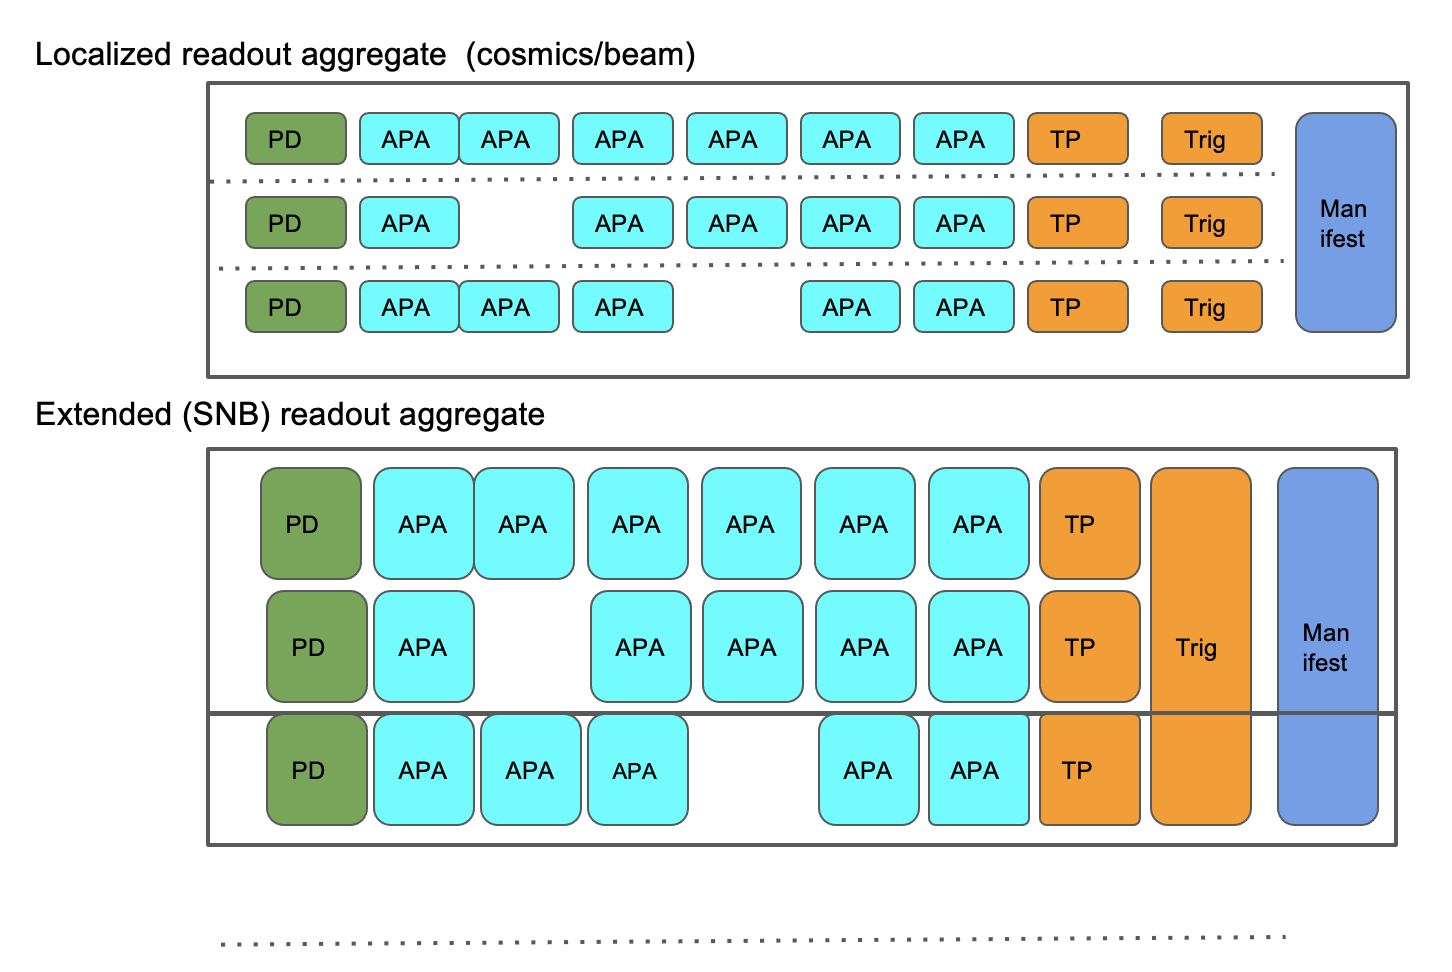
\includegraphics[width=0.8\textwidth]{graphics/IntroFigures/DataAggregation.png}
% \end{dunefigure}
% %\pagebreak

% \todo{Need more text on this case}

 
% \section{ND Beam Data: Beam data acquisition and reconstruction \hideme{ Mathew Muether/Tom Junk - needed}}
% \label{sec:use:ndbeam}  %% fix label according to section



% \section{DUNE Simulation \hideme{Junk/Schellman/Muether}}  \fixme{Mathews' diagram} 

% ND and FD data should be simulated using similar tools, differing in the detector layout but not the underlying generators. 

% \hideme\subsection{Need Mathew's diagram of the processing chain}

%\todo{how big are events?  what are memory/CPU requirements}

% \subsection{Beam simulation\hideme{Junk-draft}}\label{sec:use:beamsim}
% The neutrino beam is simulated using g4lbnf\cite{g4lbnf} a geant4\cite{geant4} based simulation of the beamline components.  Intermediate interactions are stored so that cross section reweighting can be applied.  The beam simulation is generally done separately and beam files are stored and used when needed. 

%\subsection{Cosmic simulation?}



% The far and near detectors subtend very different solid angles so one has to simulate a very large number of events or use reweighting techniques to properly cover both. 

% %\subsection{Cosmic simulation?}

% \subsection{Interaction simulation\hideme{Schellman-draft}}\label{sec:use:intmodel}
% Next an event generator is used to simulate the primary interaction.  This step requires a reasonably accurate geometry for the detectors to account for different target materials and, for the near detector, different locations. Simulation parameters and reasonably detailed event information need to be stored to allow for subsequent reweighting.  To date, most DUNE simulations have used the GENIE\cite{GENIE} event generator. 

% \subsection{Particle tracing\hideme{Junk-draft}}\label{sec:use:tracing}
% The geant4 simulation package is then used to simulate the energy deposited by final state particles as they pass through the detector.  Both ionization and scintillation signatures need to be recorded.  

% \subsection{Detector response simulation\hideme{Schellman-draft}}\label{sec:use:detsim}
% Once geant4 has simulated the energy deposit, detailed simulation of charge and light collection and electronics response can be done.  

% \subsection{Overlay\hideme{Schellman-draft}}\label{sec:use:overlay}
% It is often useful to overlay real data on simulated events to fully account for cosmic ray and upstream neutrino interactions. This adds complexity as the real data must be delivered to simulation jobs and be properly matched to the running conditions for the simulation.  The "electronics" signals from real data and simulation need to be mixed and stored.  The \dword{microboone} experiment has adapted \dword{larsoft} to do this and we plan to build on that experience. 

% \todo{Discussion of overlay experience from MicroBooNE \hideme{Kirby -needed}}

% \subsection{Reconstruction} \label{sec:use:mcreco}
% Reconstruction and analysis can then be performed using the same methods as in section \ref{sec:use:pdii}.  Due to the large amount of interaction and intermediate step information kept for studies, simulated events are often several times the size of real data.  A significant question, given the size of events, is whether it may be more efficient to regenerate than to store all the information needed for reweighting. 

% \subsection{Resource requirements for simulation and reconstruction \hideme{Schellman-Junk -needed}}
% \todo{add a table showing \# of events, CPU and memory footprint for each step}









% \section{Oscillation analysis} Chris Backhouse?  Chris Marshall? 
% \label{sec:use:osc}

% \section{Supernova data: acquisition and fast reconstruction}
% \label{sec:use:supernova}  %% fix label according to section

% \subsection{Fast ( 1 day turnaround)} \fixme{Priority for readout?}

% \subsection{Full Supernova}

% \section{Solar/BSM analysis}
% \label{sec:use:BSManalysis}

% \section{Calibration data: acquisition, reconstruction and use}
% \label{sec:use:calib}  %% fix label according to section

% \section{Hardware database use case} \fixme{Paul has an example}
% \label{sec:use:hdb} 

% \section{Analysis Facility}\todo{Claire}
% \label{sec:use:analysis}

% \section{What's missing?}
% \label{sec:use:todo}
% } % end of ignore
% \section{Data movement}
% An important component in computing is data placement.  DUNE will generate 30 PB/year and takes advantage of storage and CPU at multiple sites worldwide.  Our present model uses the Fermilab SAM system to track data locations.  Going forward, the Rucio\cite{Barisits:2019fyl} system will be used to move and locate large datasets (of order 100 TB) at DUNE storage sites.  The workflow and data dispatcher systems will then help users and processes find the most accessible copy of the data for their site. 

% \todo{Produce table that shows, input/output/CPU and memory footprint for each stage of processing - Heidi gathers info}



\end{document} % if using subfiles